As mentioned in ~\ref{sec: motivation}, a python tool is developed for this work. This chapter highlights its structure and elaborates on the details of implementation. Besides, several optimization strategies are discussed for the improvement of performance and memory usage.

\section{Why python?}

There are mainly two reasons for choosing Python over other compiled languages:

\begin{itemize}
    \item \textbf{Rapid Prototyping}: The fact that Python supports high-level language features makes it simpler to write code and to focus on readability and maintainability. This facilitates rapid prototyping in the scope of this thesis.
    \item \textbf{Rich Libraries Support}: Python has rich libraries support, including file I/O, parsing ELF file, parsing command line options, and matching patterns with regular expressions. As described more in the following sections, all of these libraries are helpful.
\end{itemize}


\section{Workflow}

\definecolor{codegreen}{rgb}{0,0.6,0}
\definecolor{codegray}{rgb}{0.5,0.5,0.5}
\definecolor{codepurple}{rgb}{0.58,0,0.82}
\definecolor{backcolour}{rgb}{0.95,0.95,0.92}

\lstdefinestyle{mystyle}{
    backgroundcolor=\color{backcolour},   
    commentstyle=\color{codegreen},
    keywordstyle=\color{magenta},
    numberstyle=\tiny\color{codegray},
    stringstyle=\color{codepurple},
    basicstyle=\ttfamily\footnotesize,
    breakatwhitespace=false,         
    breaklines=true,                 
    captionpos=b,                    
    keepspaces=true,                 
    numbers=left,                    
    numbersep=5pt,                  
    showspaces=false,                
    showstringspaces=false,
    showtabs=false,                  
    tabsize=2
}

Fig~\ref{fig:analyzer_structure} illustrates its structure. An \texttt{Analyzer} object instance takes an ELF file and its ETISS-generated instruction trace as inputs. The \texttt{Analyzer} internals (1) extract information from ELF file, (2) construct dynamic basic blocks, (3) aggregate callgrind inclusive costs, and (4) convert to callgrind output format file. 

\medskip
\dirtree{%
.1 TraceAnalysis/.
.2 main.py.
.2 lib/.
.3 \_\_init\_\_.py.
.3 analyzer.py.
.3 basicBlock.py.
}
\medskip

\begin{figure}
    \centering
    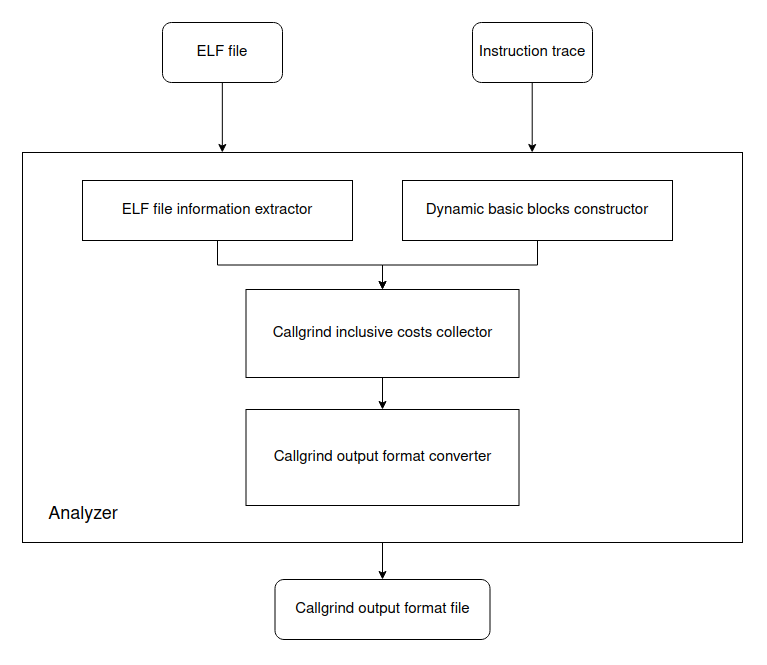
\includegraphics[width=\linewidth]{figures/Analyzer_structure.png}
    \caption{Workflow}
    \label{fig:analyzer_structure}
\end{figure}


\subsection{ELF File Information Extraction} 
\label{subsec: elf_info_extraction}

The first thing happens inside \texttt{Analyzer} internals is extracting information from ELF. Specifically, we need (1) the mapping between static program and dynamic traces and, depending on command line, (2) the mapping between program counter and source line.

\subsubsection{Static Program - Dynamic Traces Mapping}

Static program and dynamic traces are high-level terms. Concretely, we need the mapping between function and program counter range. In python, there is a well-developed library called \textit{pyelftools}, which is for parsing and analyzing ELF and DWARF debug information.~\cite{pyelftools_manual} ~\ref{code:func_pc_mapping}

With this mapping at hand, the utility function below is able to query for the function that a program counter of interest belongs to, which is extensively used in ~\ref{subsec:bb_construction} and in ~\ref{subsec:converter}.

\lstset{style=mystyle}

\begin{lstlisting}[language=Python, caption={Function that extracts static program - dynamic traces mapping}, label=code:func_pc_mapping]
from elftools.elf.elffile import ELFFile

def extract_func_to_pc_mapping(self):
    with open(self.elf_file_path, 'rb') as f:
        elffile = ELFFile(f)

        for section in elffile.iter_sections():
            if section.name == '.symtab':
                symbol_table = section
                break

        for symbol in symbol_table.iter_symbols():
            symbol_type = symbol['st_info']['type']
            if symbol_type = "STT_FUNC":
                start_pc = symbol['st_value']
                end_pc = start_pc + symbol['st_size'] - 1
                self.mapping[symbol.name] = (start_pc, end_pc)

\end{lstlisting}

\medskip
\begin{algorithm}
\caption{Utility function}
\begin{algorithmic}
\REQUIRE $pc$, program counter
\REQUIRE $mapping$, mapping between function and program counter range
\FOR{$function$ in $mapping$}
    \IF{$function\_start\_pc \leq pc \leq function\_end\_pc$}
        \RETURN $function\_name$
    \ELSE
        \RETURN $None$
    \ENDIF
\ENDFOR
\end{algorithmic}
\end{algorithm}
\medskip

\subsubsection{Program Counter - Source Line Mapping}

As mentioned in \ref{subsec:kcachegrind}, kcachegrind supports source code annotations. It is not a must but an optional feature. The tool is capable of generating \textit{callgrind output format} file ready for this feature. This is achieved by extracting the mapping between program counter and corresponding source code from input ELF file. In \ref{subsec:line_table} we briefly discuss about the information stored in \texttt{.debug\_line} ELF section. And this is all we need. The code in \label{code:debug_line_mapping} uses \textit{pyelftools} to extract the mapping for each compilation unit and store all of them in python dictionary.

\medskip
 
\begin{lstlisting}[language=Python, caption={Function that extracts mapping between program counter and source code}, label=code:debug_line_mapping]
from elftools.elf.elffile import ELFFile

def extract_pc_to_source_line_mapping(self):
    with open(self.elf_file_path, 'rb') as f:
        elffile = ELFFile(f)

        dwarfinfo = elffile.get_dwarf_info()

        for CU in dwarfinfo.iter_CUs():
            line_program = dwarfinfo.line_program_for_CU(CU)
            if line_program is None:
                continue

            CU_name = CU.get_top_DIE().attributes['DW_AT_name'].value.decode('utf-8')

            for entry in line_program.get_entries():
                if entry.state:
                    pc = entry.state.address
                    line = entry.state.line
                    self.pc_to_source_line_mapping[CU_name].append((pc, line))
                    

\end{lstlisting}

\subsection{Dynamic Basic Blocks Construction}
\label{subsec:bb_construction}

Besides to ELF file, the tool requires user to specify instruction trace file of application program. In particular, the trace generated from ETISS plugin is of the format:  

\begin{lstlisting}
program_counter: instruction_name # binary_encoding_of_instruction operand_field    
\end{lstlisting}

The workflow is shown in \ref{alg:dynamic_basic_blocks}. First, \texttt{program counter} and \texttt{instruction name} are parsed from the given line in trace file by using python \texttt{re} library. For ETISS-generated trace, the usage of \texttt{re} looks like the following:

\medskip
\begin{lstlisting}
pattern = r'(0x[0-9a-fA-F]+):\s*(\w+)\s*#\s*([0-9a-fA-F]+)'
match = re.search(pattern, line) # line in trace file
if match:
    pc = match.group(1)
    instruction = match.group(2)
\end{lstlisting}
\medskip

Afterwards, \texttt{instruction} is checked whether it is one of branch instructions. As for \textit{rv32im\_ilp32} toolchain, there are \texttt{jalr}, \texttt{jal}, \texttt{beq}, \texttt{bne}, \texttt{blt}, \texttt{bge}, \texttt{bltu}, \texttt{bgeu}. If it is true, an instance of class \texttt{BasicBlock} is constructed. It is worth noticing that the design of  \texttt{BasicBlock} object serves the purpose of compressing information of instruction level and providing a larger granularity. Moreover, it is not \textbf{static basic block} but \textbf{dynamic basic block}. Fig \ref{fig:basic_block} provides an example. 

\medskip
\begin{algorithm}
\caption{Dynamic Basic Blocks Construction}
\label{alg:dynamic_basic_blocks}
\begin{algorithmic}
\REQUIRE $dynamic\_basic\_blocks\_list$
\REQUIRE $instruction\_trace$
\FOR{$line$ in $instruction\_trace$}
    \STATE parse $program\_counter$ and $instruction\_name$ from $line$ 
    \IF{$instruction\_name$ is branch instruction name}
        \STATE construct a dynamic basic block instance
        \STATE append the instance into $dynamic\_basic\_blocks\_list$
    \ENDIF
\ENDFOR
\end{algorithmic}
\end{algorithm}
\medskip

\begin{figure}
    \centering
    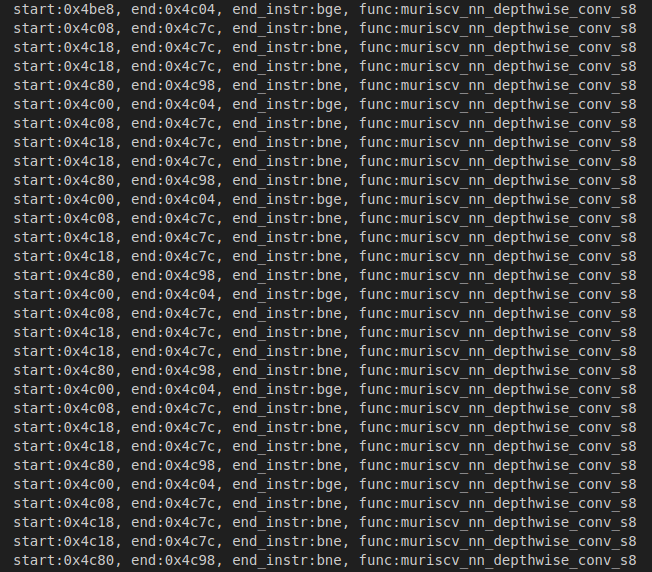
\includegraphics[width=\linewidth]{figures/Basic_Block.png}
    \caption{Example of dynamic basic blocks}
    \label{fig:basic_block}
\end{figure}

\subsection{Callgrind Inclusive Costs Collector}
                    
\subsection{Callgrind Output Format Converter}
\label{subsec:converter}

\section{Optimization}